\subsection{Experiment 4: Characteristics of Metrics in Regression Tasks}

\begin{figure}[H]
    \centering
    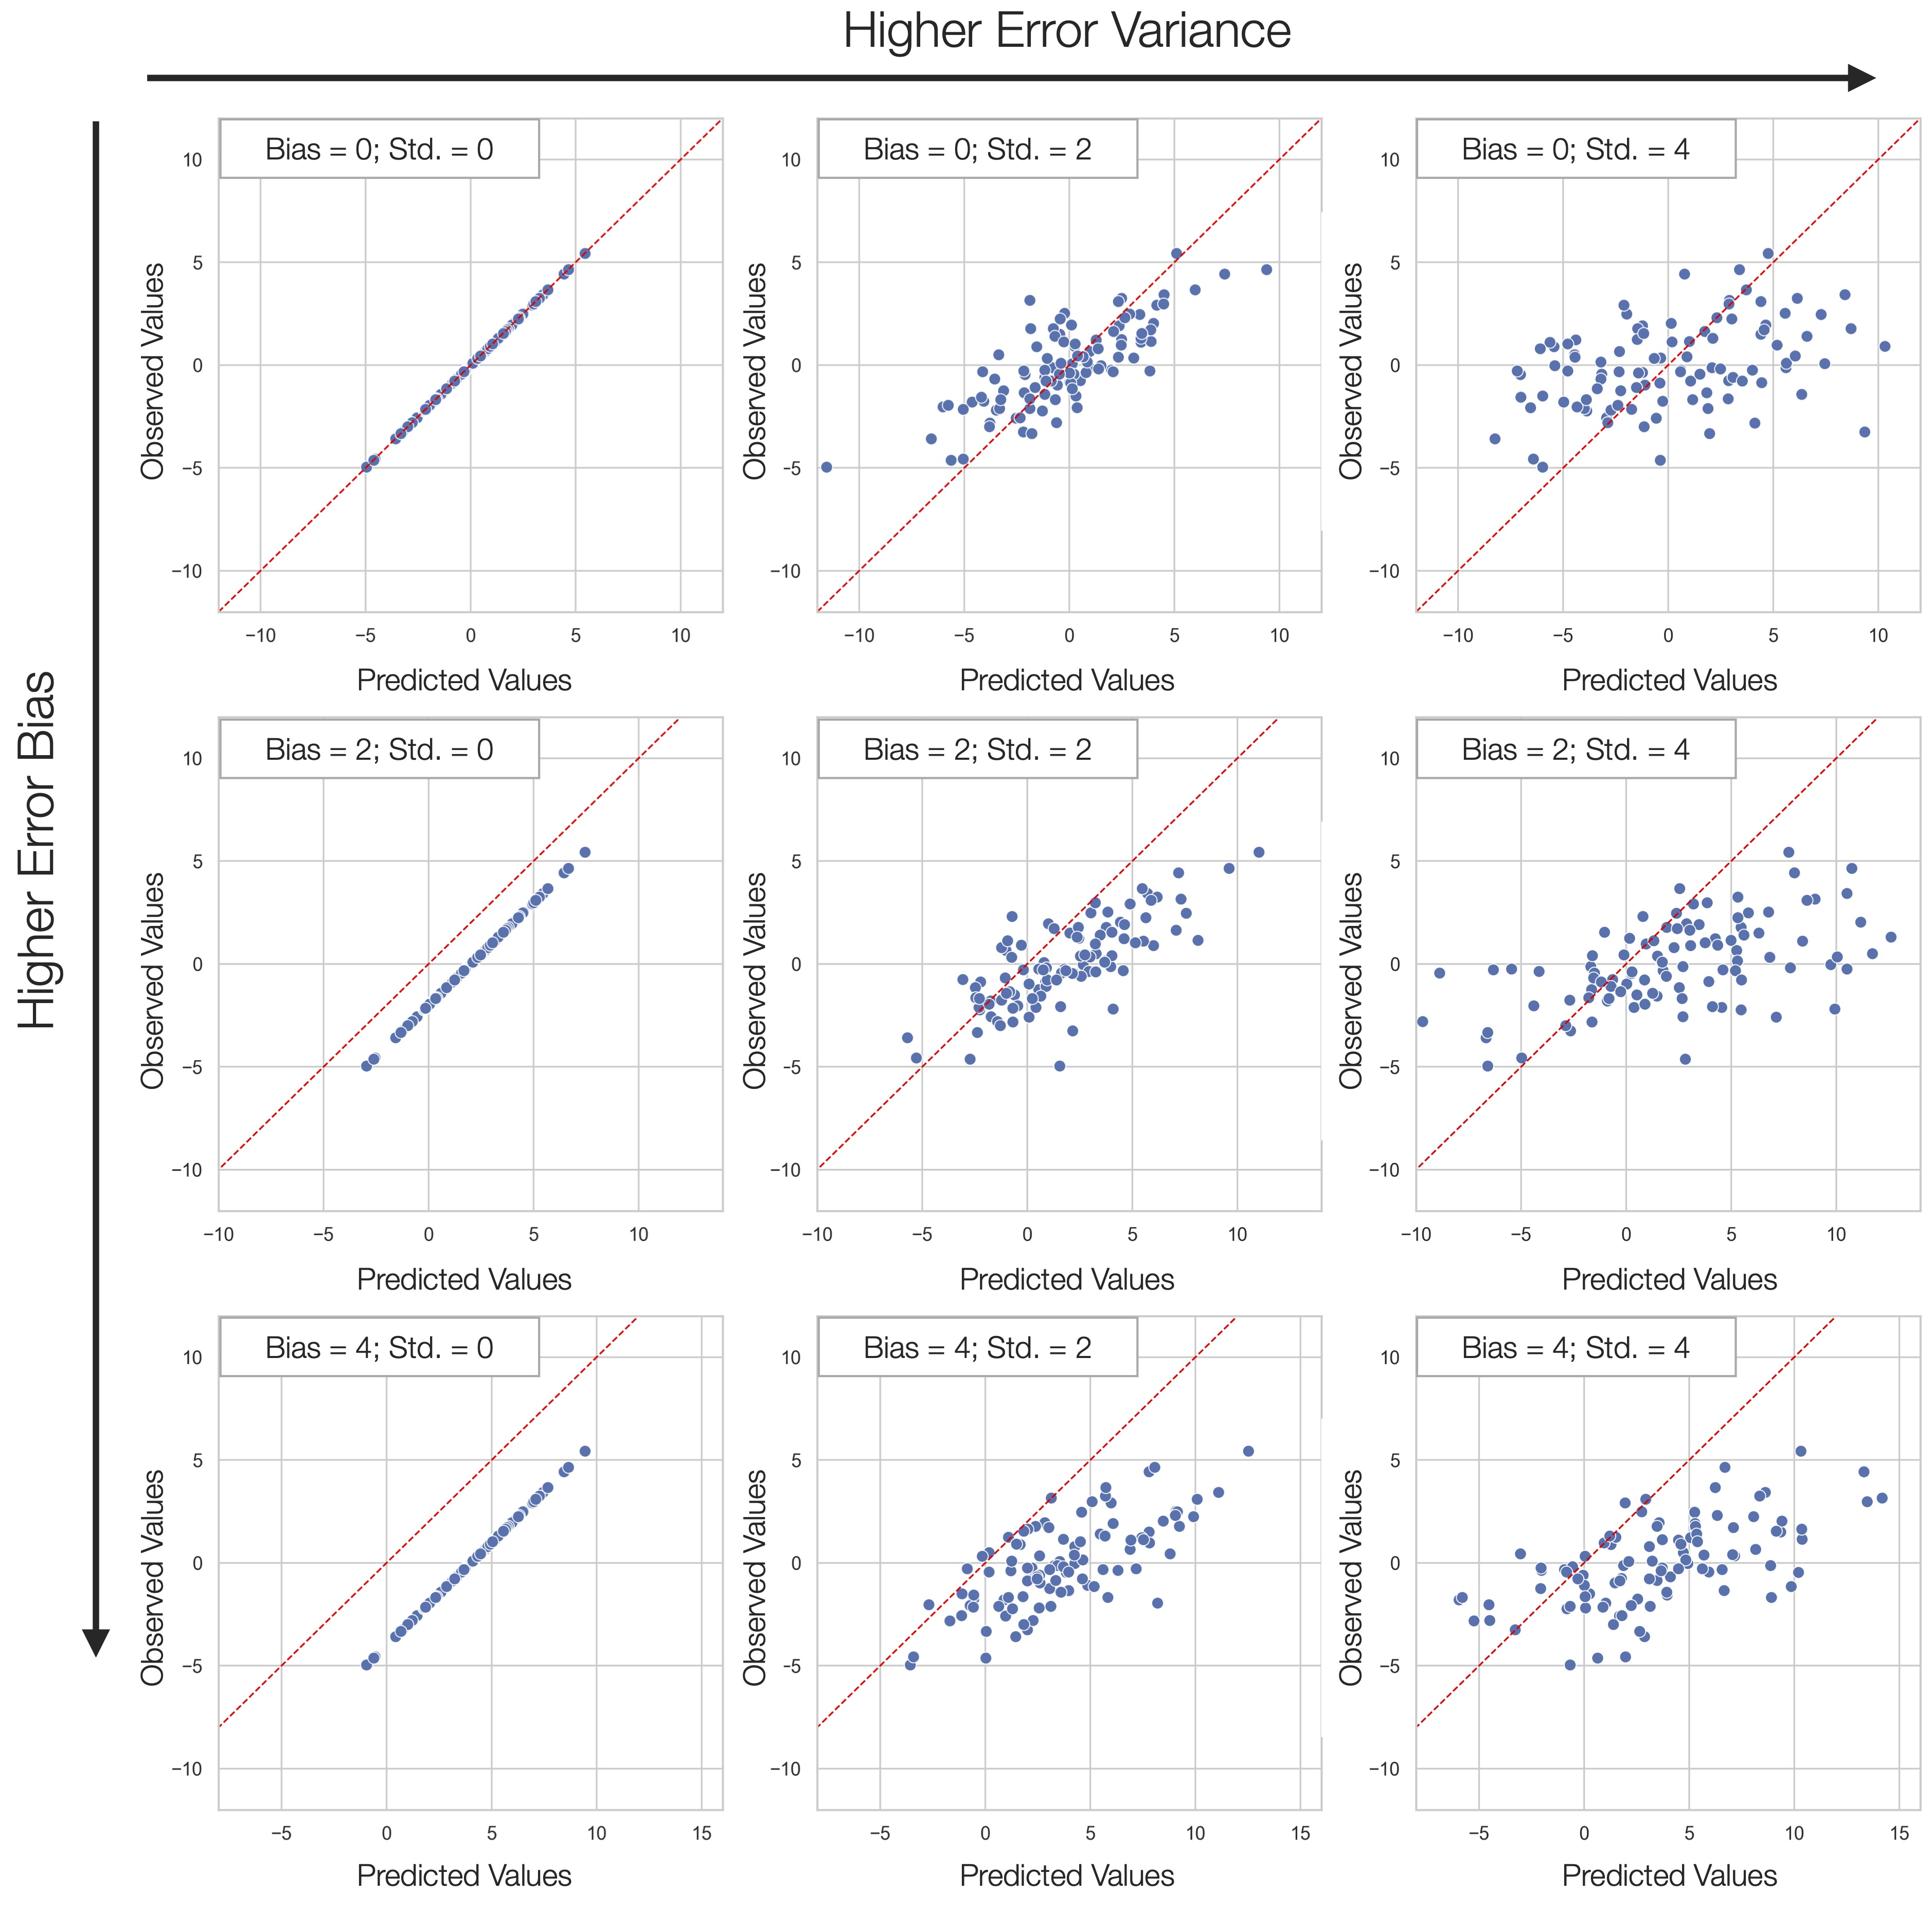
\includegraphics[width=1\textwidth]{fig_4.jpg}
    \caption{Scatter plots illustrating the relationship between predicted and actual values for 9 combinations of bias and variance, with each parameter set to one of three levels: 0, 2, or 4. The red diagonal line represents the ideal prediction line.}
    \label{fig:s4_regression}
\end{figure}

The objective of this experiment is to examine how different performance metrics in regression tasks respond to two types of prediction errors: bias and variance. The experiment aims to highlight the unique characteristics of each metric, such as sensitivity to outliers or systematic bias, and provide guidance for selecting appropriate metrics in regression tasks. Additionally, it seeks to verify the trade-off relationship between bias and variance in prediction errors.

To achieve this, six levels of bias and variance are examined: $[0, 0.5, 1, 2, 4, 8]$, forming a total of 36 combinations of prediction errors. The bias error can be considered as a systematic error that consistently overestimates or underestimates the ground truth values, while the variance error represents the random fluctuations around the ground truth. Outliers of prediction errors are considered as extreme cases of variance errors, where the predicted values deviate considerably from the ground truth. The simulated ground truth values are generated from a normal distribution with a mean of 0 and a standard deviation of 2, while the predicted values ($\hat{y}$) are created by adding random errors ($\epsilon$) with specified levels of bias and variance to the ground truth:

\begin{equation}
\begin{cases}
y \sim \mathcal{N}(0, 2) \\
\epsilon \sim \mathcal{N}(b, s) \\
\hat{y} = y + \epsilon
\end{cases}
\end{equation}

where $b$ represents the bias and $s$ represents the variance of the prediction errors (Figure ~\ref{fig:s4_regression}). The choice of a standard deviation of 2 for the ground truth values is intended to highlight the differences in behavior between the RMSE and RSR metrics, with RSR being standardized by the standard deviation of the ground truth values while RMSE tracks the original error scale.


The evaluated metrics in this experiment are categorized into two main groups. Error-based metrics include RMSE, MAE, and RSR. These metrics focus on quantifying the magnitude of errors in the predictions. Linearity-based metrics, such as $r$, $R^2$, and CCC, assess the linear relationship and agreement between the predicted and actual values. By systematically exploring how each metric responds to varying levels of bias and variance, this experiment demonstrates their strengths, limitations, and practical implications for regression analysis. The findings are intended to guide practitioners in selecting the most appropriate performance metrics based on their specific modeling objectives and the characteristics of their data.

